
WRITE MORE about provenance of python code: \url{https://github.com/romaguir/sph_models}

There are several datasets available:
\begin{itemize}
\item {\sl GypSum\_S.sph}: Simmons et al (2010) \cite{sifb10}
\item {\sl S20RTS.sph}, {\sl S40RTS.sph}:  Ritsema et al (2011) \cite{ridv11} 
      website\footnote{\url{https://jritsema.earth.lsa.umich.edu/Research.html}}
\item {\sl s362ani\_m\_s.sph}: Kustowski et al (2008) \cite{kued08}
\item {\sl SEM\_WM\_s.sph}: French \& Romanowicz (2015) \cite{frro15}
\item {\sl GAP\_P4.sph}: Obayashi et al (2013) \cite{obyn13,fuob13} 
      website\footnote{\url{http://d-earth.jamstec.go.jp/GAP_P4/}}
%\item {\sl SP12RTS..EC.sph}: \cite{kord16}
%\item {\sl SP12RTS..EP.sph}:  \cite{kord16}
%\item {\sl SP12RTS..ES.sph}:  \cite{kord16}
\end{itemize}

All at 100km depth:
\begin{center}
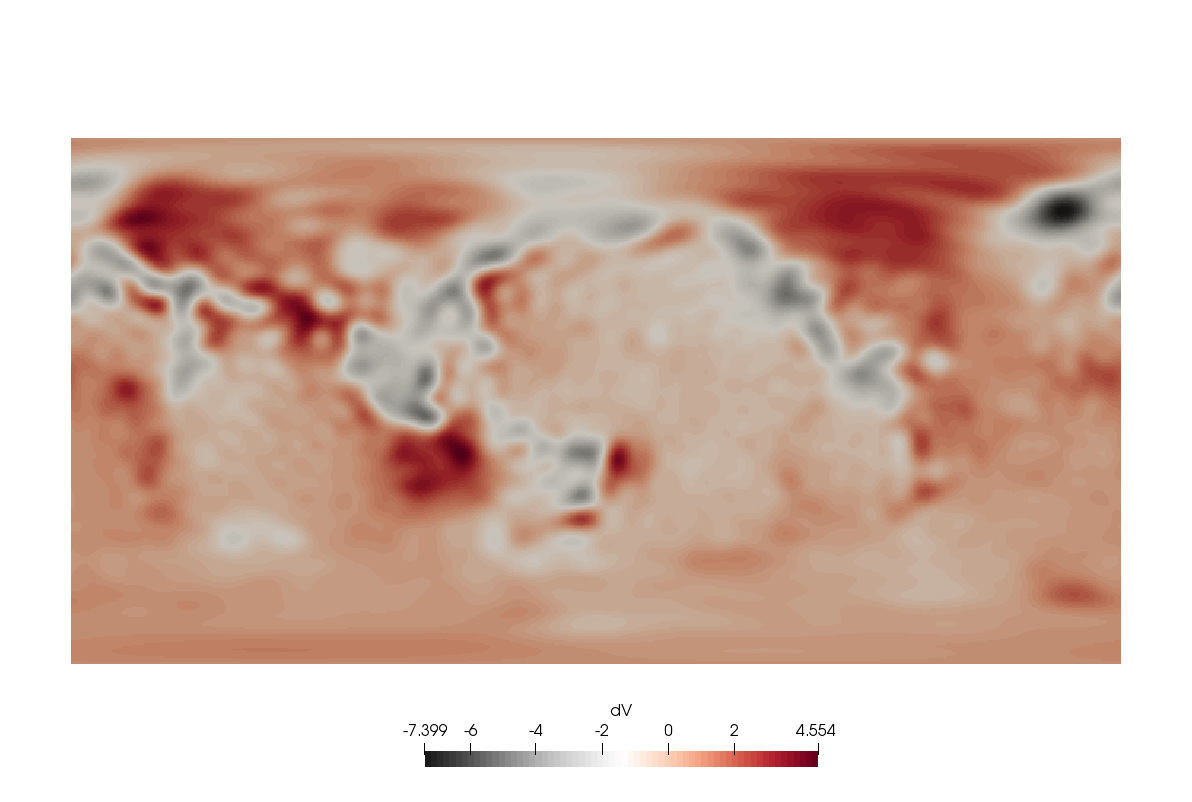
\includegraphics[width=7cm]{python_codes/fieldstone_66/images/GAP_P4}
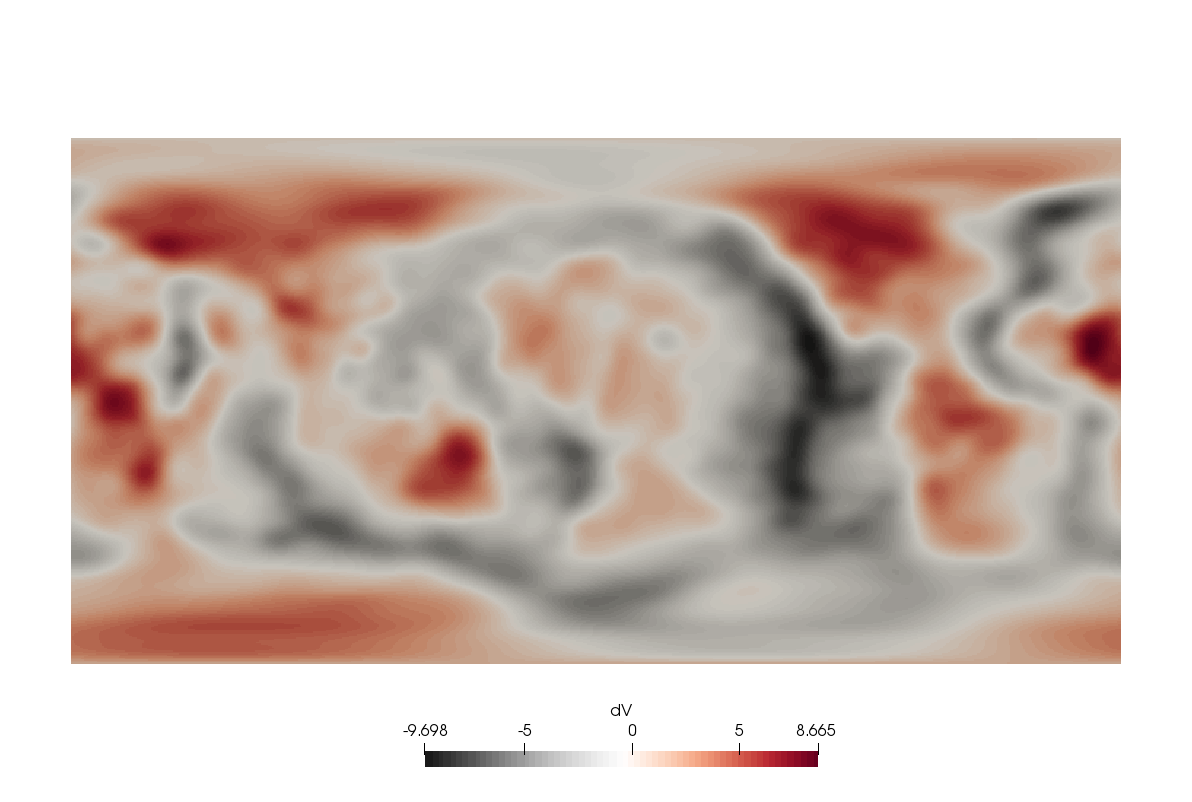
\includegraphics[width=7cm]{python_codes/fieldstone_66/images/GyPSum_S}\\
GAP\_P4 $\uparrow$ \hspace{7cm} GyPSum $\uparrow$ \\
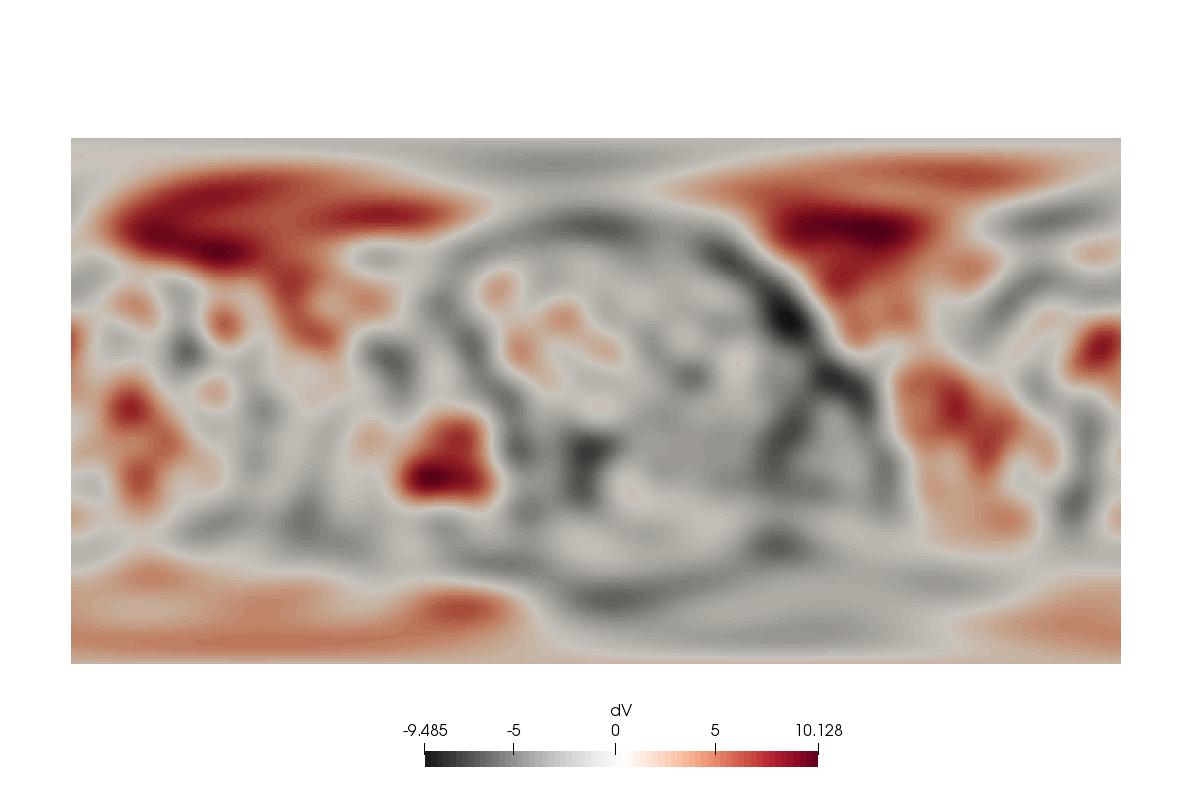
\includegraphics[width=7cm]{python_codes/fieldstone_66/images/S20RTS}
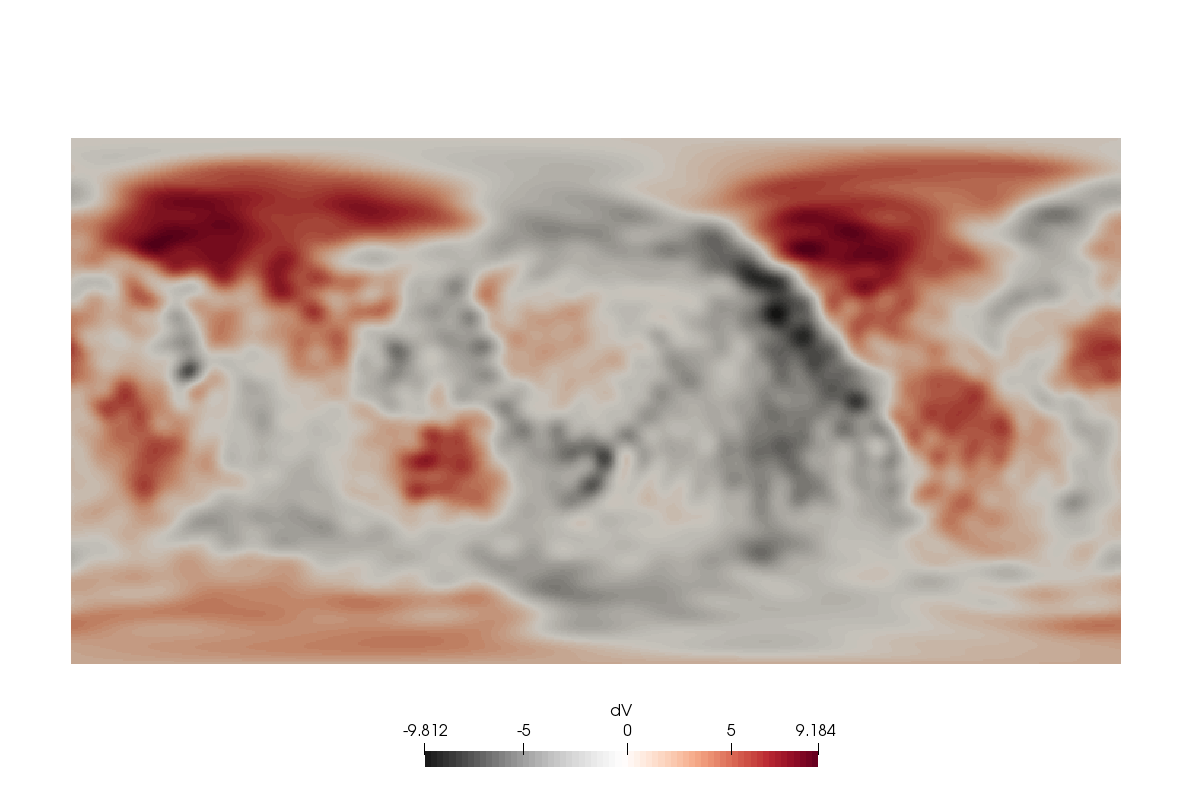
\includegraphics[width=7cm]{python_codes/fieldstone_66/images/S40RTS}\\
S20RTS $\uparrow$ \hspace{7cm} S40RTS $\uparrow$ \\
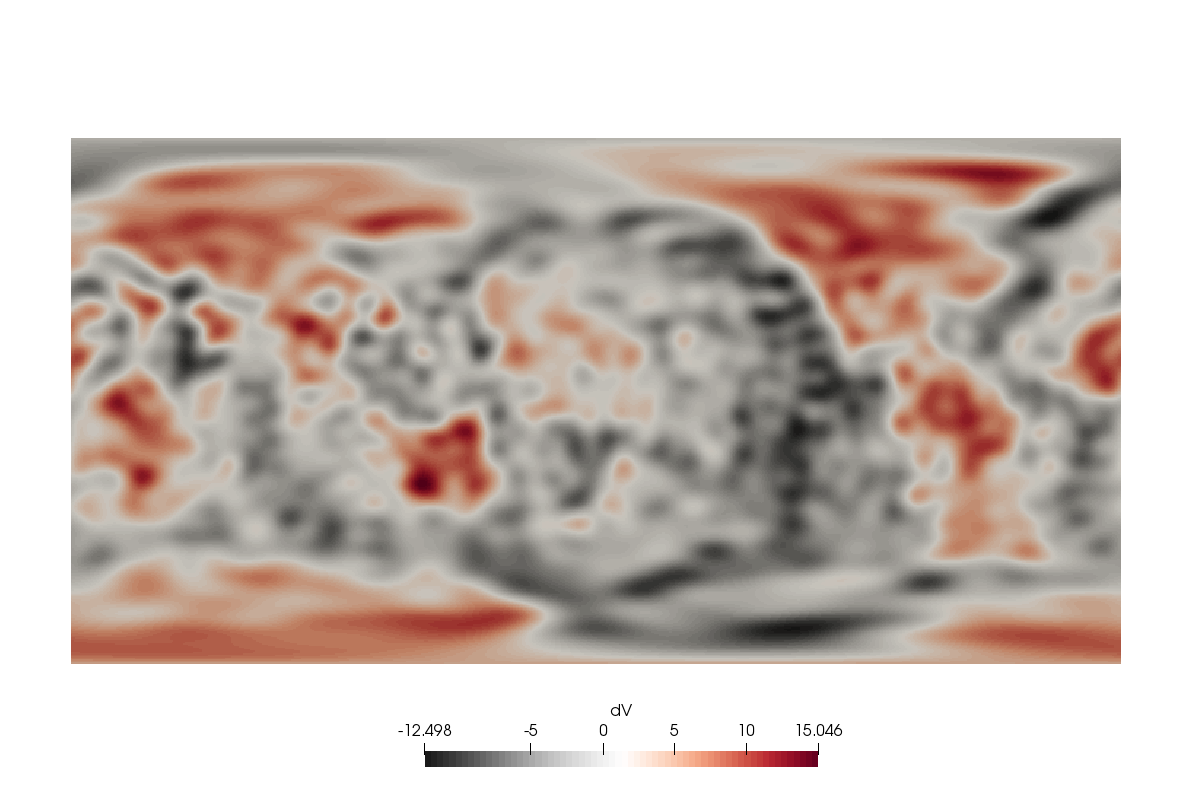
\includegraphics[width=7cm]{python_codes/fieldstone_66/images/SEM_WM_s}
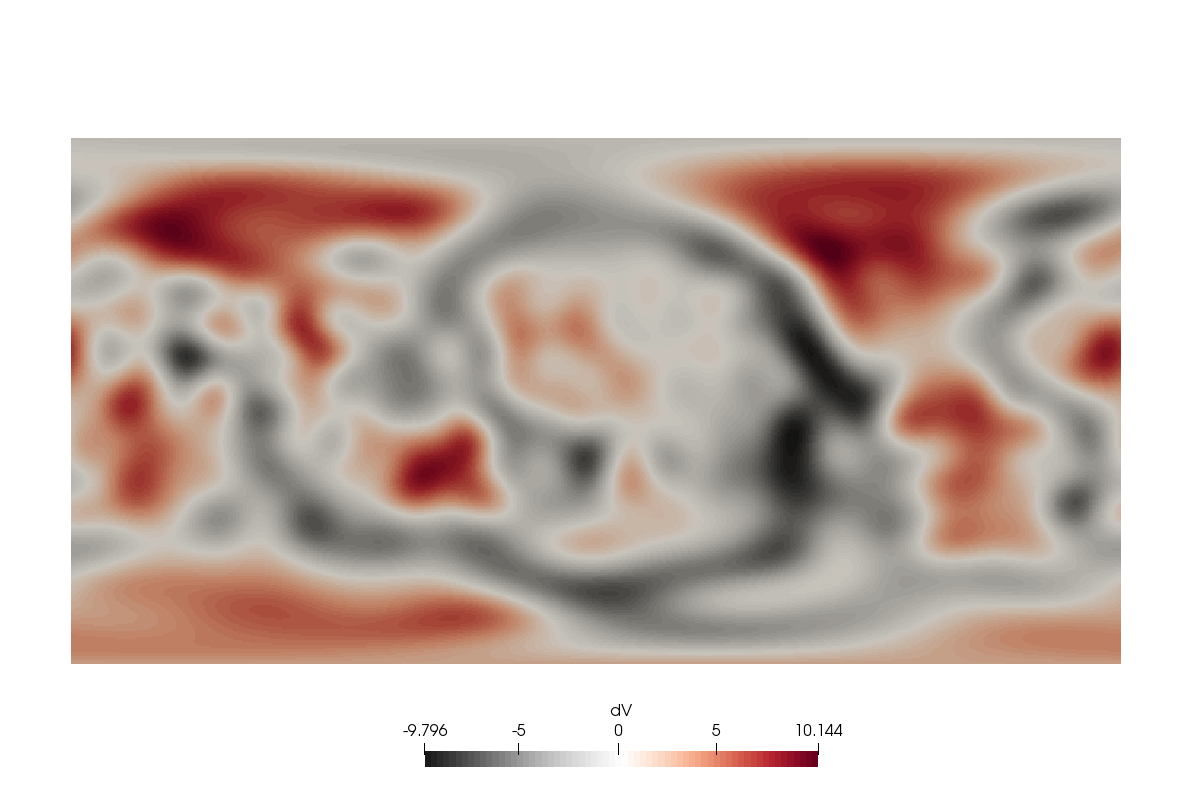
\includegraphics[width=7cm]{python_codes/fieldstone_66/images/s362ani_m_s}\\
SEM\_WM $\uparrow$ \hspace{7cm} S362ANI $\uparrow$\\
\end{center}


\begin{center}
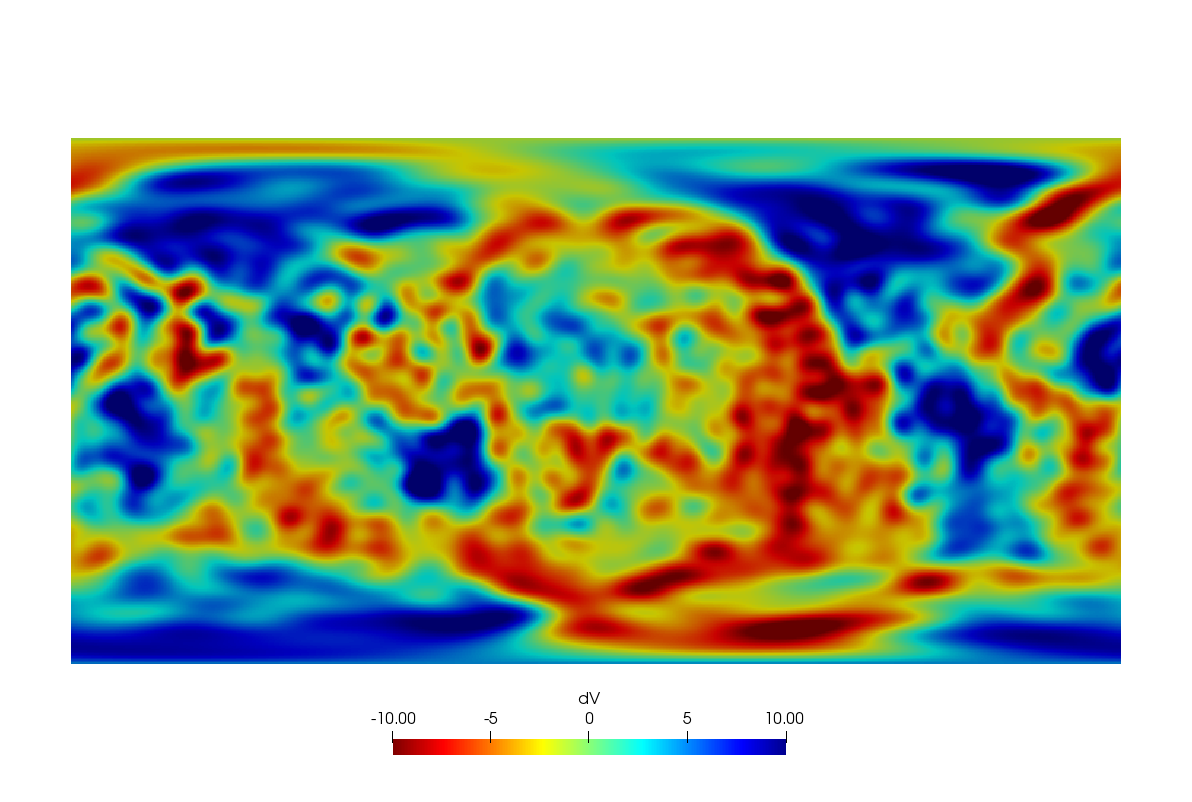
\includegraphics[width=7cm]{python_codes/fieldstone_66/images/SEM_WM_s2}
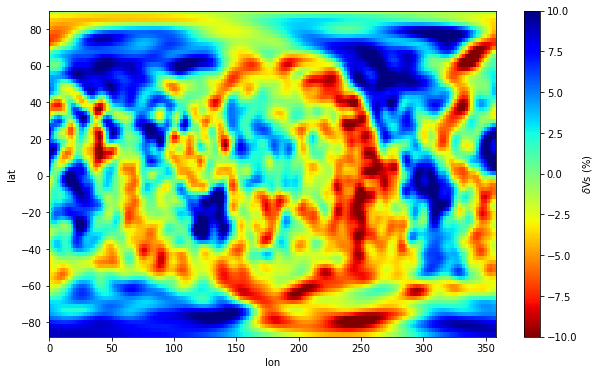
\includegraphics[width=7cm]{python_codes/fieldstone_66/images/SEM_WS_notebook}\\
{\captionfont SEM\_WM. Left: fieldstone; Right: as shown in notebook.} 
\end{center}

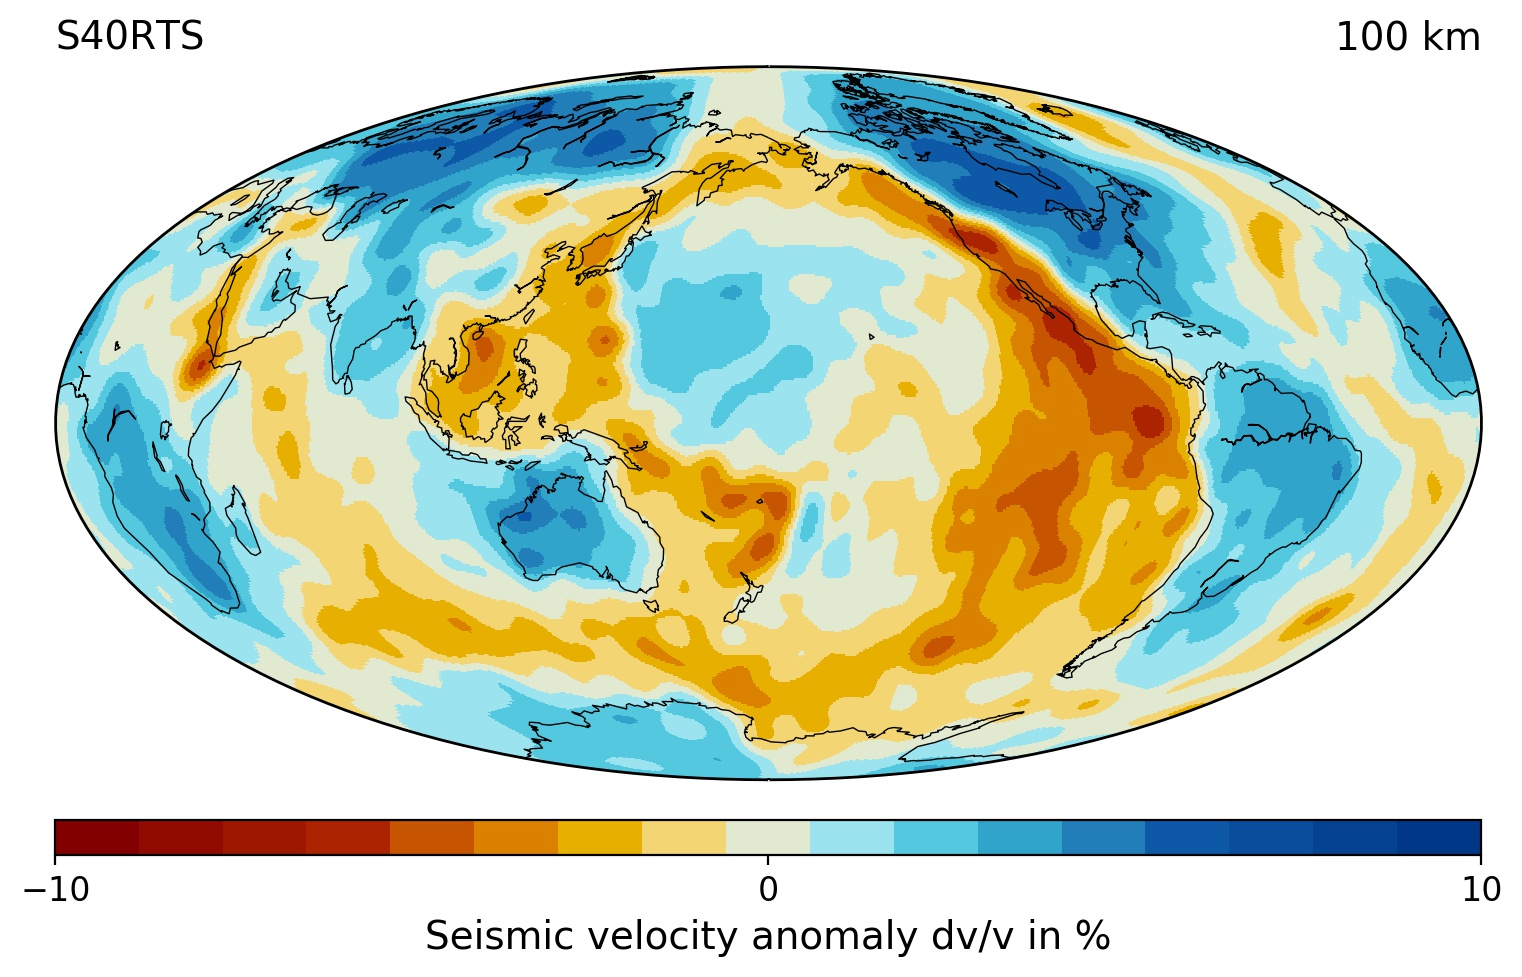
\includegraphics[width=7cm]{python_codes/fieldstone_66/images/S40RTS_tomo_depth}
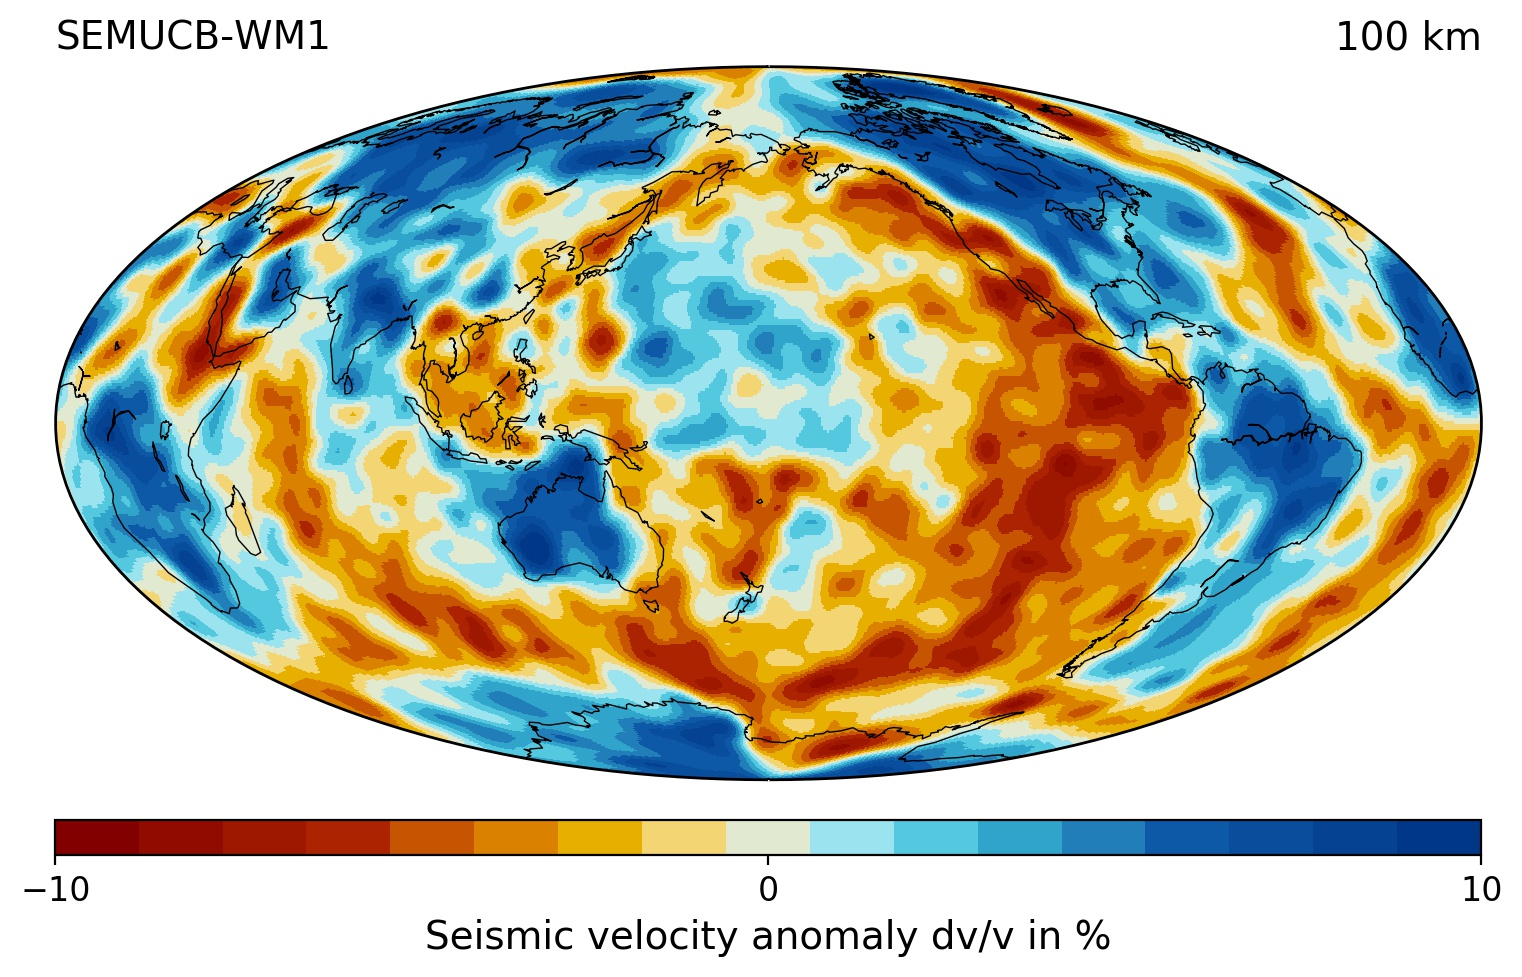
\includegraphics[width=7cm]{python_codes/fieldstone_66/images/SEMUCB-WM1_tomo_depth}

